\mysection{Hacker l'horloge de Windows}

Parfois je fais des poissons d'avril à mes collègues.

Cherchons si nous pourrions faire quelque chose avec l'horloge de Windows?
Pouvons-nous la forcer à tourner à l'envers?

Tout d'abord, lorsque l'on clique sur date/time dans la barre d'état,\\
le module \emph{C:\textbackslash{}WINDOWS\textbackslash{}SYSTEM32\textbackslash{}TIMEDATE.CPL}
est exécuté, qui est un fichier exécutable \ac{PE} habituel.

Voyons d'abord comment il affiche les aiguilles.
Lorsque j'ouvre le fichier (de Windows 7) dans Resource Hacker, il y a le fond de
l'horloge, mais sans aiguille:

\begin{figure}[H]
\centering
\myincludegraphics{examples/timedate/reshack.png}
\caption{Resource Hacker}
\end{figure}

Ok, que savons-nous? Comment afficher une aiguille? Elles commencent au milieu du
cercle, s'arrêtent sur son bord.
De ce fait, nous devons calculer les coordonnées d'un point sur le bord d'un cercle.
Des mathématiques scolaires, nous pouvons nous rappeler que nous devons utiliser
les fonctions sinus/cosinus pour dessiner un cercle, ou au moins la racine carré.
Il n'y a pas de telles choses dans \emph{TIMEDATE.CPL}, au moins à première vue.
Mais grâce au fichier PDB de débogage de Microsoft, je peux trouver une fonction
appelée \emph{CAnalogClock::DrawHand()}, qui appelle \emph{Gdiplus::Graphics::DrawLine()}
au moins deux fois.

Voici le code:

\lstinputlisting[style=customasmx86]{examples/timedate/1.lst}

\myindex{Windows!Win32!MulDiv()}
Nous voyons que les arguments de \emph{DrawLine()} dépendent du résultat de la fonction
\emph{MulDiv()} et d'une table \emph{table[]} (le nom est mien), qui a des éléments
de 8-octets (regardez le second opérande de \INS{LEA}).

Qu'y a-t-il dans table[]?

\lstinputlisting[style=customasmx86]{examples/timedate/2.lst}

Elle n'est référencée que depuis la fonction \emph{DrawHand()}.
Elle a 120 mots de 32-bit ou 60 paires 32-bit... attendez, 60?
Regardons ces valeurs de plus près.
Tout d'abord, je vais remplacer 6 paires ou 12 mots de 32-bit par des zéros, et je
vais mettre le fichier \emph{TIMEDATE.CPL} modifié dans \emph{C:\textbackslash{}WINDOWS\textbackslash{}SYSTEM32}.
(Vous pourriez devoir changer le propriétaire du fichier *TIMEDATE.CPL* pour votre
compte utilisateur primaire (au lieu de \emph{TrustedInstaller}), et donc, démarrer
en mode sans échec avec la ligne de commande afin de pouvoir copier le fichier, qui
est en général bloqué.)

\begin{figure}[H]
\centering
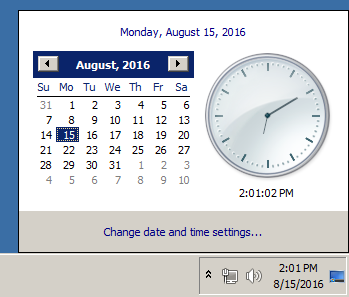
\includegraphics[width=0.5\textwidth]{examples/timedate/6_pairs_zeroed.png}
\caption{Tentative d'exécution}
\end{figure}

Maintenant lorsqu'une aiguilles est située dans 0..5 secondes/minutes, elle est invisible!
Toutefois, la partie opposée (plus courte) de la seconde aiguille est visible et
bouge.
Lorsqu'une aiguille est en dehors de cette partie, elle est visible comme d'habitude.

\myindex{Mathematica}
Regardons d' encore plus près la table dans Mathematica.
J'ai copié/collé la table de \emph{TIMEDATE.CPL} dans un fichier \emph{tbl} (480 octets).
Nous tenons pour acquis le fait que ce sont des valeurs signées, car la moitié des
éléments sont inférieurs à zéro (0FFFFE0C1h, etc.).
Si ces valeurs étaient non signées, elles seraient étrangement grandes.

\begin{lstlisting}[style=custommath]
In[]:= tbl = BinaryReadList["~/.../tbl", "Integer32"]

Out[]= {0, -7999, 836, -7956, 1663, -7825, 2472, -7608, 3253, -7308, 3999, \
-6928, 4702, -6472, 5353, -5945, 5945, -5353, 6472, -4702, 6928, \
-4000, 7308, -3253, 7608, -2472, 7825, -1663, 7956, -836, 8000, 0, \
7956, 836, 7825, 1663, 7608, 2472, 7308, 3253, 6928, 4000, 6472, \
4702, 5945, 5353, 5353, 5945, 4702, 6472, 3999, 6928, 3253, 7308, \
2472, 7608, 1663, 7825, 836, 7956, 0, 7999, -836, 7956, -1663, 7825, \
-2472, 7608, -3253, 7308, -4000, 6928, -4702, 6472, -5353, 5945, \
-5945, 5353, -6472, 4702, -6928, 3999, -7308, 3253, -7608, 2472, \
-7825, 1663, -7956, 836, -7999, 0, -7956, -836, -7825, -1663, -7608, \
-2472, -7308, -3253, -6928, -4000, -6472, -4702, -5945, -5353, -5353, \
-5945, -4702, -6472, -3999, -6928, -3253, -7308, -2472, -7608, -1663, \
-7825, -836, -7956}

In[]:= Length[tbl]
Out[]= 120
\end{lstlisting}

Traitons deux valeurs consécutives comme une paire:

\begin{lstlisting}[style=custommath]
In[]:= pairs = Partition[tbl, 2]
Out[]= {{0, -7999}, {836, -7956}, {1663, -7825}, {2472, -7608}, \
{3253, -7308}, {3999, -6928}, {4702, -6472}, {5353, -5945}, {5945, \
-5353}, {6472, -4702}, {6928, -4000}, {7308, -3253}, {7608, -2472}, \
{7825, -1663}, {7956, -836}, {8000, 0}, {7956, 836}, {7825, 
1663}, {7608, 2472}, {7308, 3253}, {6928, 4000}, {6472, 
4702}, {5945, 5353}, {5353, 5945}, {4702, 6472}, {3999, 
6928}, {3253, 7308}, {2472, 7608}, {1663, 7825}, {836, 7956}, {0, 
7999}, {-836, 7956}, {-1663, 7825}, {-2472, 7608}, {-3253, 
7308}, {-4000, 6928}, {-4702, 6472}, {-5353, 5945}, {-5945, 
5353}, {-6472, 4702}, {-6928, 3999}, {-7308, 3253}, {-7608, 
2472}, {-7825, 1663}, {-7956, 836}, {-7999, 
0}, {-7956, -836}, {-7825, -1663}, {-7608, -2472}, {-7308, -3253}, \
{-6928, -4000}, {-6472, -4702}, {-5945, -5353}, {-5353, -5945}, \
{-4702, -6472}, {-3999, -6928}, {-3253, -7308}, {-2472, -7608}, \
{-1663, -7825}, {-836, -7956}}

In[]:= Length[pairs]
Out[]= 60
\end{lstlisting}

Essayons de traiter chaque paire comme des coordonnées X/Y et dessinons les 60 paires,
et aussi les 15 premières paires:

\begin{figure}[H]
\centering
\myincludegraphics{examples/timedate/math.png}
\caption{Mathematica}
\end{figure}

Ça donne quelque chose!
Chaque paire est juste une coordonnée.
Les 15 premières paires sont les coordonnées pour $\frac{1}{4}$ de cercle.

Peut-être que les développeurs de Microsoft ont pré-calculé toutes les coordonnées
et les ont mises dans une table.
myindex{Memoization}
Ceci est une pratique très répandue, quoique désuète -- l'accès à une table précalculée
est plus rapide que d'appeler les fonctions sinus/cosinus relativement lente\footnote{Aujourd'hui
ceci est appelé la \emph{memoïsation}}.
Les opérations sinus/cosinus ne sont plus aussi couteuses...

Maintenant, je comprends pourquoi lorsque j'ai effacé les 6 premières paires, les
aiguilles étaient invisibles dans cette zone: en fait, les aiguilles étaient dessinées,
elles avaient juste une longueur de zéro, car elles commençaient et finissaient en (0,0).

\subsubsection{La blague}

Sachant tout cela, comment serait-il possible de forcer les aiguilles à tourner à
l'envers?
En fait, ceci est simple, nous devons seulement tourner la table, afin que chaque
aiguille, au lieu d'être dessinée à l'index 0, le soit à l'index 59.

J'ai créé le modificateur il y a longtemps, au tout début des années 2000, pour Windows 2000.
Difficile à croire, il fonctionne toujours pour Windows 7, peut-être que la table
n'a pas changé depuis lors!

Code source du modificateur: \url{\RepoURL/examples/timedate/time_pt.c}.

Maintenant, je peux voir les aiguilles tourner à l'envers:

\begin{figure}[H]
\centering
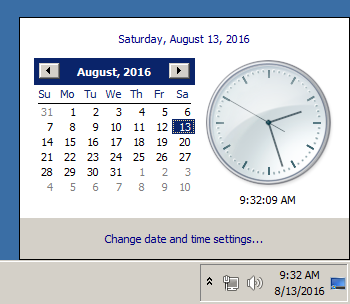
\includegraphics[width=0.5\textwidth]{examples/timedate/counterclockwise.png}
\caption{Maintenant ça fonctionne}
\end{figure}

Bon, il n'y a pas d'animation dans ce livre, mais si vous y regardez de plus près,
vous pouvez voir que les aiguilles affichent en fait l'heure correcte, mais que la
surface entière de l'horloge est tournée verticalement, comme si nous la voyons depuis
l'intérieur de l'horloge.

\subsubsection{Code source divulgué de Windows 2000}

Donc, j'ai écrit le modificateur et ensuite le code source de Windows 2000 a fuité
(je ne peux toutefois pas vous obligez à me croire).
Jettons un coup d'\oe{}il au code source de cette fonction et à la table.\\
Le fichier est \emph{win2k/private/shell/cpls/utc/clock.c}:

\begin{lstlisting}[style=customc]
//
//  Array containing the sine and cosine values for hand positions.
//
POINT rCircleTable[] =
{
    { 0,     -7999},
    { 836,   -7956},
    { 1663,  -7825},
    { 2472,  -7608},
    { 3253,  -7308},
...
    { -4702, -6472},
    { -3999, -6928},
    { -3253, -7308},
    { -2472, -7608},
    { -1663, -7825},
    { -836 , -7956},
};

////////////////////////////////////////////////////////////////////////////
//
//  DrawHand
//
//  Draws the hands of the clock.
//
////////////////////////////////////////////////////////////////////////////

void DrawHand(
    HDC hDC,
    int pos,
    HPEN hPen,
    int scale,
    int patMode,
    PCLOCKSTR np)
{
    LPPOINT lppt;
    int radius;

    MoveTo(hDC, np->clockCenter.x, np->clockCenter.y);
    radius = MulDiv(np->clockRadius, scale, 100);
    lppt = rCircleTable + pos;
    SetROP2(hDC, patMode);
    SelectObject(hDC, hPen);

    LineTo( hDC,
            np->clockCenter.x + MulDiv(lppt->x, radius, 8000),
            np->clockCenter.y + MulDiv(lppt->y, radius, 8000) );
}
\end{lstlisting}

Maintenant, c'est clair: les coordonnées sont pré-calculées comme si la surface de
l'horloge avait une hauteur et une largeur de $2 \cdot 8000$, et ensuite elles sont
adaptées au rayon actuel de l'horloge en utilisant la fonction \emph{MulDiv()}.

La structure POINT\footnote{\url{https://msdn.microsoft.com/en-us/library/windows/desktop/dd162805(v=vs.85).aspx}}
est une structure de deux valeurs 32-bit, la première est \emph{x}, la seconde \emph{y}.

